\documentclass{beamer}
\usepackage{tikz}
\usepackage{amsmath}
\usetikzlibrary{shapes.geometric, arrows, positioning}

\title{Sensor Fusion: Integrating IMU and ArUco-Based GPS}
\subtitle{MAE 162E Capstone}
\author{Jimmy Yang, Po-Chih (Toby) Chen, Ting-Hao (Jason) Liu, Shuo-Wu (Will) Shih}
\date{April 15, 2026}

\begin{document}

\frame{\titlepage}

\begin{frame}{Background and Motivation}
    \textbf{Goal:} Determine the precise pose (position and orientation) of the robot for planning and navigation through the obstacle course.
    \vspace{0.5cm}
    \begin{itemize}
        \item \textbf{Current Stage:} The robot is able to navigate through a series of waypoints using dead reckoning (pose estimation from wheel odometry), but the accumulated drift causes it to deviate from the intended path over time.
        \item \textbf{The Problem:} Wheel slippage and encoder quantization cause accumulated drift over time.
        \item \textbf{The Solution:} Sensor fusion combines high-frequency odometry with absolute external sensors to produce an optimal estimate.
    \end{itemize}
\end{frame}


\begin{frame}{Sensor Modalities and Limitations}
    \begin{itemize}
        \item \textbf{Wheel Odometry (100 Hz)}
        \begin{itemize}
            \item \textit{Measurement:} Pose $\mathbf{p}_{\text{odom}}, \theta_{\text{odom}}$ from wheel encoders using differential drive kinematics.
            \item \textit{Advantage:} High update rate gives smooth local trajectory however subject to unbounded drift over long distances.
        \end{itemize}
        \item \textbf{Inertial Measurement Unit (IMU) (25 Hz)}
        \begin{itemize}
            \item \textit{Advantage:} Absolute heading reference via magnetometer and gravity vector.
            \item \textit{Limitation:} Lower update rate, subject to noise and magnetic interference from motors/cables.
        \end{itemize}
        \item \textbf{ArUco-Based GPS (10 Hz)}
        \begin{itemize}
            \item \textit{Advantage:} Absolute position $\mathbf{p}_{\text{GPS}}$  in the arena frame (offset to produce position in the global frame).
            \item \textit{Limitation:} Lower update rate, subject to camera occlusion and latency.
        \end{itemize}
    \end{itemize}
\end{frame}

\begin{frame}{The Complementary Filter}
    A weighted-sum filter nudges the smooth odometry estimate toward the absolute sensor reading at every timestep.
    \vspace{0.5cm}
    
    \textbf{Orientation Fusion:}
    \begin{equation*}
        \hat{\theta}_{\text{fused}} = \theta_{\text{odom}} + \alpha \cdot \text{wrap}(\theta_{\text{imu}} - \theta_{\text{odom}})
    \end{equation*}
    \textit{Note: \texttt{wrap()} folds the angle difference into $[-\pi, +\pi]$ to prevent discontinuities.}
    
    \vspace{0.5cm}
    \textbf{Position Fusion:}
    \begin{equation*}
        \hat{\mathbf{p}}_{\text{fused}} = \mathbf{p}_{\text{odom}} + \alpha_{\text{pos}} \cdot (\mathbf{p}_{\text{GPS}} - \mathbf{p}_{\text{odom}})
    \end{equation*}
\end{frame}

\begin{frame}{Filter Tuning Parameters}
    The tuning parameters ($\alpha_{\text{orientation}}$ and $\alpha_{\text{pos}}$) determine the trust ratio between sensors, defined on the interval $[0,1]$.

    \vspace{0.3cm}
    \begin{itemize}
        \item \textbf{$\alpha = 0$:} Pure odometry (no external correction).
        \item \textbf{$\alpha = 1$:} Pure absolute sensor (snaps to reading every tick, highly noisy).
        \item \textbf{Small $\alpha$ (e.g., 0.02):} Gentle long-term drift correction. The absolute sensor slowly pulls the estimate toward the truth without introducing moment-to-moment control noise.
    \end{itemize}

    \vspace{0.3cm}
    \textbf{Note:} \texttt{ORIENTATION\_ALPHA = 0.0} in \texttt{robot.py} for the actual robot run --- the IMU magnetometer is disrupted by motor magnetic fields in the current lab.  Task~1a is a learning exercise only; do not enable orientation fusion for the course run.
\end{frame}

\begin{frame}{ROS 2 Software Architecture}
    \centering
    \resizebox{0.9\linewidth}{!}{%
    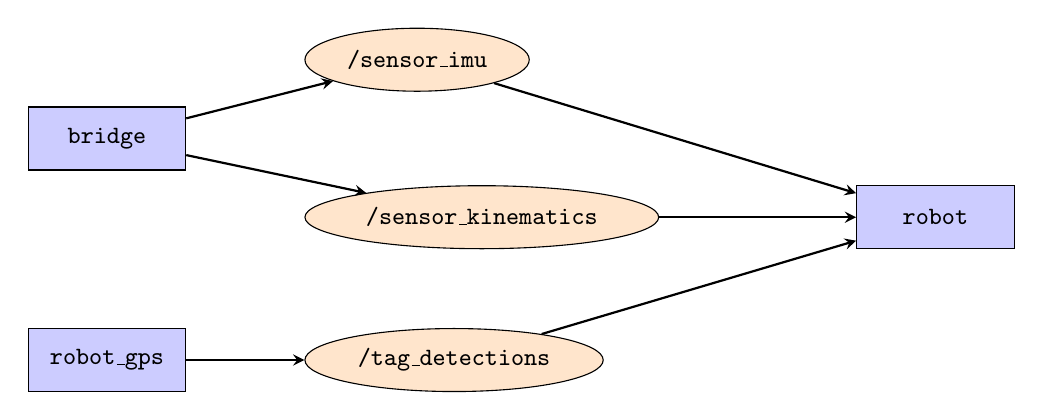
\begin{tikzpicture}[
        node distance=1.5cm and 2cm,
        box/.style={rectangle, draw, fill=blue!20, minimum width=2cm, minimum height=0.8cm, text centered, font=\small},
        topic/.style={ellipse, draw, fill=orange!20, minimum width=2.5cm, minimum height=0.8cm, text centered, font=\small},
        arrow/.style={thick,->,>=stealth}
    ]
        % Left Column (Publishers)
        \node[box] (bridge) {\texttt{bridge}};
        \node[box, below=2cm of bridge] (robotgps) {\texttt{robot\_gps}};
        
        % Middle Column (Topics)
        \node[topic, right=1.5cm of bridge, yshift=1cm] (imu) {\texttt{/sensor\_imu}};
        \node[topic, right=1.5cm of bridge, yshift=-1cm] (kinematics) {\texttt{/sensor\_kinematics}};
        \node[topic, right=1.5cm of robotgps] (tag) {\texttt{/tag\_detections}};
        
        % Right Column (Subscribers)
        % Anchoring 'robot' to the right of 'kinematics' guarantees no overlap
        \node[box, right=2.5cm of kinematics] (robot) {\texttt{robot}};
        
        % Edges
        \draw[arrow] (bridge) -- (imu);
        \draw[arrow] (bridge) -- (kinematics);
        \draw[arrow] (robotgps) -- (tag);
        
        \draw[arrow] (imu) -- (robot);
        \draw[arrow] (kinematics) -- (robot);
        \draw[arrow] (tag) -- (robot);
        
    \end{tikzpicture}%
    }
    
    \vspace{0.4cm}
    \begin{itemize}
        \item \textbf{\texttt{/sensor\_kinematics}:} Wheel odometry at 25 Hz from the Arduino.
        \item \textbf{\texttt{/sensor\_imu}:} IMU orientation data from the Arduino.
        \item \textbf{\texttt{/tag\_detections}:} Location of tags from the ArUco GPS detections.
    \end{itemize}
\end{frame}

\begin{frame}{Coordinate Frames \& GPS Alignment}
    \begin{itemize}
        \item \textbf{World/Arena Frame:} Origin $(0,0)$ at corner anchor~0; $x$-axis toward corner~1; $y$-axis toward corner~2 (toward the ramp).
        \item \textbf{Starting orientation:} Robot must face the positive $y$ direction (toward the ramp) $\Rightarrow$ \texttt{INITIAL\_THETA\_DEG = 90.0} in \texttt{main.py}.  No change needed if placed correctly at the taped start.
        \item \textbf{GPS offset:} Pre-measured for the venue and already set in \texttt{test\_position\_fusion.py} and \texttt{main.py}. \textbf{Do not change.}
        \begin{itemize}
            \item \texttt{GPS\_OFFSET\_X\_MM = 609.6}
            \item \texttt{GPS\_OFFSET\_Y\_MM = -304.8}
        \end{itemize}
        \item \textbf{Dead-Reckoning Fallback:} If the ArUco tag is occluded, the system dead-reckons from the last valid GPS fix using the odometry delta.
    \end{itemize}
\end{frame}

\begin{frame}[fragile]{Commands for Fusion Tuning}
    \textbf{Terminal 1 (inside Docker) --- start bridge every time:}
    \begin{verbatim}
docker compose -f ros2_ws/docker/docker-compose.rpi.yml up -d
docker compose exec ros2_runtime bash
ros2 run bridge bridge
    \end{verbatim}

    \textbf{Terminal 2 (inside Docker) --- run the desired test:}
    \begin{verbatim}
docker compose exec ros2_runtime bash
ros2 launch robot test_position_fusion.launch.py
# or
ros2 launch robot test_orientation_fusion.launch.py
    \end{verbatim}

    \textbf{Viewing results (outside Docker, in VS Code terminal):}
    \begin{itemize}
        \item Position fusion: image already in \texttt{\textasciitilde/Project-NUEVO/} --- Ctrl-click to open.
        \item Orientation fusion / trajectory: copy first, then Ctrl-click:
    \end{itemize}
    \begin{verbatim}
docker cp docker-ros2_runtime-1:/root/orientation_fusion_test_result.png \
    ~/Project-NUEVO/
docker cp docker-ros2_runtime-1:/ros2_ws/trajectory.png ~/Project-NUEVO/
    \end{verbatim}
\end{frame}

\begin{frame}{What to Tune in Each Test}
    \begin{itemize}
        \item \textbf{Position fusion:} edit \texttt{POSITION\_ALPHA} in \texttt{robot.py} (class constant), then relaunch.
        \item \textbf{Orientation fusion (learning exercise):} edit \texttt{FUSION\_ALPHA} in \texttt{test\_orientation\_fusion.py}. This does \emph{not} affect the actual robot run (\texttt{ORIENTATION\_ALPHA = 0.0} in \texttt{robot.py}).
        \item \textbf{Position test workflow:} robot drives 1000~mm straight; saves \texttt{position\_fusion\_test\_result.png} directly to \texttt{\textasciitilde/Project-NUEVO/}.
        \item \textbf{Orientation test workflow:} robot drives two circles; result saved inside Docker --- requires \texttt{docker cp} to view.
        \item \textbf{For the course run:} set \texttt{TAG\_ID} in \texttt{main.py} and tune \texttt{POSITION\_ALPHA} in \texttt{robot.py}.  Everything else can stay at its default.
    \end{itemize}
\end{frame}

\begin{frame}{Key Parameters Reference}
    \begin{tabular}{lll}
        \hline
        \textbf{Parameter} & \textbf{File} & \textbf{Action} \\
        \hline
        \texttt{TAG\_ID} & \texttt{main.py} & Set to your group's assigned tag ID \\
        \texttt{POSITION\_ALPHA} & \texttt{robot.py} & Tune (0.0--1.0); default 0.10 \\
        \texttt{ORIENTATION\_ALPHA} & \texttt{robot.py} & Leave at 0.0 (IMU unreliable) \\
        \texttt{INITIAL\_THETA\_DEG} & \texttt{main.py} & Leave at 90.0 (face $+y$, toward ramp) \\
        \texttt{TAG\_X\_OFFSET\_MM} & \texttt{robot.py} & 0.0 if tag centred on axle midpoint \\
        \texttt{TAG\_Y\_OFFSET\_MM} & \texttt{robot.py} & 0.0 if tag centred on axle midpoint \\
        \texttt{IMU\_Z\_DOWN} & \texttt{robot.py} & False (chip faces up); optional \\
        \texttt{GPS\_OFFSET\_X/Y} & \texttt{main.py} & Pre-set --- do not change \\
        \hline
    \end{tabular}

    \vspace{0.4cm}
    \textbf{ArUco tag mounting tips:}
    \begin{itemize}
        \item Mount flat; sides of printed square parallel to robot axes.
        \item Centre tag above the midpoint of the drive-wheel axle line.
        \item Tilt or rotation causes systematic position/heading errors.
    \end{itemize}
\end{frame}

\begin{frame}{Visual Alpha-Tuning Checklist}
    \textbf{Position fusion}
    \begin{itemize}
        \item If fused Y barely corrects back toward the floor markers, raise $\alpha_{\text{pos}}$.
        \item If the fused path snaps sideways or chatters when GPS is active, lower $\alpha_{\text{pos}}$.
        \item If GPS is never acquired, the run is not useful for alpha tuning.
    \end{itemize}

    \vspace{0.2cm}
    \textbf{Orientation fusion}
    \begin{itemize}
        \item If fused heading nearly matches odometry throughout, $\alpha_{\text{orientation}}$ is too low.
        \item If fused heading is jagged or noisy while odometry is smooth, $\alpha_{\text{orientation}}$ is too high.
        \item A good result keeps the correction bounded and smooth during the spin.
    \end{itemize}
\end{frame}

\begin{frame}{Dead Reckoning vs. Sensor Fusion}
    \centering
    % TODO: Upload your plot and change 'localization_plot.png' to your filename
    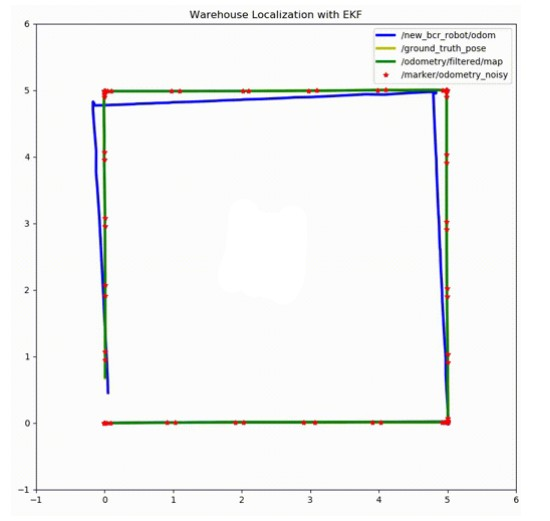
\includegraphics[width=0.5\textwidth]{figures/dead_reckoning_vs_sensor_fusion.jpg}
    
    \vspace{0.3cm}
    \begin{itemize}
        \item \textbf{Blue:} Robot location based on dead reckoning (drifts over time).
        \item \textbf{Green:} Robot location based on sensor fusion (remains accurate).
    \end{itemize}
\end{frame}

\begin{frame}{Venue Navigation with Pure Pursuit}
    Accurate pose estimation enables the execution of pure-pursuit path planning.
    \vspace{0.3cm}
    \begin{enumerate}
        \item \textbf{Read Fused Pose:} Obtain $(\hat{x}, \hat{y}, \hat{\theta})$ from sensor fusion.
        \item \textbf{Advance Path:} Compare the fused pose against the waypoint list.
        \item \textbf{Compute Lookahead:} Determine the pursuit point on the path ahead of the robot.
        \item \textbf{Command Velocity:} Calculate and send linear and angular velocity commands to correct the cross-track error.
    \end{enumerate}
\end{frame}

\end{document}
